\documentclass[11pt]{article}
\usepackage[margin=1in]{geometry}
\usepackage{graphicx}
\usepackage{hyperref}
\title{Vibe Research Document Pipeline Verification}
\author{Local Reconstruction Test}
\date{July 2026}
\begin{document}
\maketitle
\begin{abstract}
This document validates a real local artifact chain: LaTeX source, a compiled PDF, a Word document, and a generated diagram image.
\end{abstract}
\section{Pipeline}
The reconstructed application invokes bundled or local document tools and preserves concrete outputs for inspection.
\begin{figure}[ht]
\centering
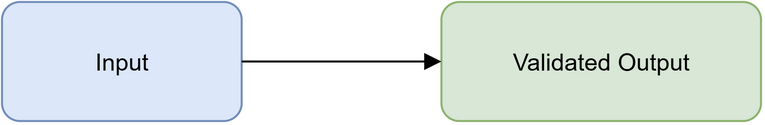
\includegraphics[width=0.75\linewidth]{../figures/pipeline.png}
\caption{Locally generated document pipeline diagram.}
\end{figure}
\section{Quality Gate}
The PDF must open, contain at least one page, embed the diagram, and contain extractable text. The DOCX must contain document XML, media, relationships, and non-empty paragraphs.
\end{document}
